% !TeX root = ../../../tesis.tex

% =============================================================================
%  SECCIÓN 3.3.9 — Clasificación Garibelt: instrumento de síntesis diagnóstica
% =============================================================================

\subsection{Clasificación Garibelt: instrumento de síntesis diagnóstica}
\label{subsec:clasificacion-garibelt}

Los ocho indicadores definidos en esta sección caracterizan la red de forma
independiente: cada uno mide una dimensión específica del grafo $\grafo$ y
produce un valor cuya unidad y escala le son propias. La
\textbf{Clasificación Garibelt} opera en un nivel distinto: no es el noveno
indicador sino un instrumento de síntesis que toma cinco de los ocho ---$C$,
$C_i$, $DI$, $T$ y $B(v)$--- y los reúne en un tablero de diagnóstico topológico
sin colapsar sus diferencias en un escalar único.

\begin{table}[htbp]
\centering
\small
\caption[Clasificación Garibelt v1: dimensiones, métodos de normalización y rangos de referencia]{%
    Clasificación Garibelt v1: cinco dimensiones con su método de normalización
    y rango de referencia para el diagnóstico topológico.}
\label{tab:clasificacion-garibelt-dims}
\begin{tabularx}{\textwidth}{>{\raggedright\arraybackslash}X c >{\raggedright\arraybackslash}l >{\raggedright\arraybackslash}X c c}
    \toprule
    \textbf{Dimensión} & \textbf{Sím.} &
    \textbf{Método de normalización} &
    \textbf{Rango de referencia} &
    \textbf{Óptimo} & \textbf{Crítico} \\
    \midrule
    Accesibilidad — Cobertura Espacial
      & $C$ & Estándar bibliográfico
      & 0\,\%–80\,\% (peatonal urbano) & 80\,\% & 0\,\% \\
    Conectividad capilar — Fuerza Capilar
      & $C_i$ & Percentil empírico
      & Q1–Q3 del dataset & Q3 & Q1 \\
    Eficiencia de ruta — Índice de Ruta Directa
      & $DI$ & Límites teóricos
      & $[1.0,\;2.5]$ & 1.0 & 2.5 \\
    Fluidez global — Tiempo de Viaje Promedio
      & $T$ & Por referencia externa
      & 85–180\,min (\textsc{enoe}/\cdmx{}) & 85\,min & 180\,min \\
    Centralidad crítica — Intermediación
      & $B(v)$ & $1 - \mathrm{Gini}(B)$
      & Rango $[0,1]$, Gini invertido & 1.0 & 0.0 \\
    \bottomrule
\end{tabularx}
\smallskip
\fuentefigura{Elaboración propia con base en \citet{talukder2017} y
\citet{bocarejo2012}.}
\end{table}

% !TeX root = ../../../tesis.tex

% =====================================================================
\subsubsection{El problema de la compensabilidad}
\label{subsubsec:garibelt-compensabilidad}
% =====================================================================

Los cinco indicadores que integra este instrumento no son cinco formas
distintas de medir lo mismo: son cinco dimensiones de un fenómeno que no
admite una unidad de medida única. La cobertura~$C$ opera sobre fracciones
del territorio; el tiempo promedio~$T$ recoge la experiencia del usuario en
minutos; la intermediación~$B(v)$ describe la posición de cada nodo en la
estructura del grafo. Reunir estas magnitudes en un solo número es
técnicamente posible, pero produce una cifra que oscurece más de lo que
revela. La Clasificación Garibelt propone una salida distinta: un tablero de
cinco lecturas donde cada dimensión conserva su propio rango y su propio
significado, y donde las diferencias estructurales permanecen visibles.

Agregar cinco indicadores en un promedio parece resolver el problema de la
heterogeneidad, pero introduce otro: el sesgo de compensabilidad. Una red
puede obtener una nota global «aceptable» si dos dimensiones son excelentes,
aunque una tercera esté en estado crítico; el promedio absorbe ese dato en
lugar de exhibirlo \citep{hossain2024}. \citet{deng2023} documentan este
riesgo en redes multimodales: la concentración de flujo en nodos clave no
queda visible en índices compuestos, y esa invisibilidad dificulta la
priorización de intervenciones. La
Figura~\ref{fig:compensabilidad-garibelt} ilustra el contraste con la
Red~$\beta$: el índice ponderado arroja $0.56$ —Aceptable— mientras el
Espectro MJG deja en primer plano la dimensión de eficiencia en estado
Crítico.

\begin{figure}[htbp]
\centering
% Diagrama: Problema de compensabilidad — Clasificación Garibelt
% Usado en: 5-Analisis-Red-Actual/5-6-Clasificacion-Garibelt/5-6-1-Fundamento.tex
% fig:compensabilidad-garibelt
%
% Muestra cómo un índice compuesto (0.56 — Aceptable) oculta la dimensión
% Crítica que el Espectro Garibelt sí deja visible.
% Colores de bandas: red!65 / orange!65 / yellow!55!green!35 / green!50
% Coordenadas diseñadas para caber en \textwidth (≈14 cm).

\begin{tikzpicture}[
    casilla/.style = {
        rectangle,
        minimum width  = 3.8cm,
        minimum height = 0.65cm,
        inner sep      = 5pt,
        align          = center,
        font           = \small,
        rounded corners= 3pt
    },
    etiq/.style = {
        font       = \small,
        align      = right,
        text width = 3.4cm
    }
]

% ================================================================
%  PANEL IZQUIERDO — índice compuesto
%  Barra de escala [0,1] con 4 bandas; marcador en 0.56
%  Barra: x in [0, 5];  y in [4.10, 4.85]
%  Bandas: 0–1.25 / 1.25–2.50 / 2.50–3.75 / 3.75–5.00
% ================================================================

\node[font=\small\bfseries, align=center] at (2.5, 5.65)
    {Índice compuesto};
\node[font=\scriptsize\itshape, color=gray!60, align=center] at (2.5, 5.25)
    {Red hipotética $\beta$};

% Bandas coloreadas
\fill[red!65]             (0.00, 4.10) rectangle (1.25, 4.85);
\fill[orange!65]          (1.25, 4.10) rectangle (2.50, 4.85);
\fill[yellow!55!green!35] (2.50, 4.10) rectangle (3.75, 4.85);
\fill[green!50]           (3.75, 4.10) rectangle (5.00, 4.85);
\draw[gray!50, thin]      (0.00, 4.10) rectangle (5.00, 4.85);
\draw[gray!55, thin] (1.25, 4.10) -- (1.25, 4.85);
\draw[gray!55, thin] (2.50, 4.10) -- (2.50, 4.85);
\draw[gray!55, thin] (3.75, 4.10) -- (3.75, 4.85);

% Etiquetas de banda
\node[font=\tiny\bfseries, white]  at (0.625, 4.475) {Crít.};
\node[font=\tiny\bfseries]         at (1.875, 4.475) {Débil};
\node[font=\tiny\bfseries]         at (3.125, 4.475) {Acept.};
\node[font=\tiny\bfseries, white]  at (4.375, 4.475) {Idón.};

% Marcador en 0.56 → x = 0.56 × 5 = 2.80
\fill[unamAzul!80]
    (2.80, 4.10) -- (2.67, 3.86) -- (2.93, 3.86) -- cycle;
\node[font=\footnotesize\bfseries, anchor=north]
    at (2.80, 3.85) {$0.56$ — Aceptable};

% Ticks de escala inferior
\foreach \xval/\lab in {0.00/0.0, 1.25/0.25, 2.50/0.50, 3.75/0.75, 5.00/1.0}{
    \draw[gray!45] (\xval, 4.10) -- (\xval, 3.97);
    \node[font=\tiny, color=gray!55, anchor=north] at (\xval, 3.97) {\lab};
}

% ================================================================
%  FLECHA CENTRAL
% ================================================================
\draw[-Stealth, thick, color=gray!45]
    (5.30, 4.48) -- (6.10, 4.48)
    node[midway, above, font=\tiny\itshape, color=gray!55] {desagregado};

% ================================================================
%  PANEL DERECHO — Espectro Garibelt
%  Labels (right-aligned, text width 3.4 cm): centradas en x = 8.0
%  Casillas (width 3.8 cm): centradas en x = 11.80
%  Filas: y = 4.90, 4.08, 3.26, 2.44, 1.62  (dy = 0.82)
% ================================================================

\node[font=\small\bfseries, align=center] at (10.30, 5.65)
    {Espectro Garibelt};
\node[font=\scriptsize\itshape, color=gray!60, align=center] at (10.30, 5.25)
    {misma Red $\beta$};

% Fila 1 — Accesibilidad 0.80 Idóneo
\node[etiq] at (8.0, 4.90) {Accesibilidad ($C$)};
\node[casilla, fill=green!50, draw=gray!40]
    at (11.80, 4.90) {$0.80$ — \textbf{Idóneo}};

% Fila 2 — Conectividad 0.75 Idóneo
\node[etiq] at (8.0, 4.08) {Conectividad ($C_i$)};
\node[casilla, fill=green!50, draw=gray!40]
    at (11.80, 4.08) {$0.75$ — \textbf{Idóneo}};

% Fila 3 — Eficiencia 0.20 Crítico (resaltada)
\node[etiq, font=\small\bfseries] at (8.0, 3.26) {Eficiencia ($DI$)};
\node[casilla, fill=red!65, text=white, draw=red!70, line width=0.8pt]
    at (11.80, 3.26) {$0.20$ — \textbf{Crítico}};

% Fila 4 — Fluidez 0.45 Débil
\node[etiq] at (8.0, 2.44) {Fluidez ($T$)};
\node[casilla, fill=orange!65, draw=gray!40]
    at (11.80, 2.44) {$0.45$ — Débil};

% Fila 5 — Centralidad 0.60 Aceptable
\node[etiq] at (8.0, 1.62) {Centralidad ($B(v)$)};
\node[casilla, fill=yellow!55!green!35, draw=gray!40]
    at (11.80, 1.62) {$0.60$ — Aceptable};

% Nota al pie del panel derecho
\node[font=\scriptsize\itshape, color=red!60,
      anchor=north, text width=4.6cm, align=center]
    at (10.30, 1.15)
    {Dimensión Crítica: visible en el espectro,\\
     oculta en el índice compuesto};

\end{tikzpicture}

\caption[Problema de compensabilidad en índices compuestos de transporte]{%
    Problema de compensabilidad en una red hipotética ($\beta$). A la
    izquierda, el índice ponderado produce $0.56$ (Aceptable), ocultando
    que la eficiencia de ruta está en estado Crítico. A la derecha, el
    Espectro MJG preserva esa información al mantener cada dimensión
    en su propia banda.}
\label{fig:compensabilidad-garibelt}
\fuentefigura{Elaboración propia. Ejemplo hipotético con fines ilustrativos.}
\end{figure}

% =====================================================================
\subsubsection{Normalización como calibración, no como agregación}
\label{subsubsec:garibelt-normalizacion}
% =====================================================================

Resolver el problema de las unidades heterogéneas no es lo mismo que
sumarlas: es calibrarlas. Llevar magnitudes distintas a una escala común
sirve para que sean comparables en un mismo tablero, no para operarlas
aritméticamente. \citet{kujala2018} construyeron un repositorio de
indicadores de redes de transporte para 25 ciudades normalizando los datos
\gtfs{} de cada una, pero sin producir un índice global: el resultado de
su trabajo es un perfil multidimensional por ciudad, precisamente porque
normalizar y agregar son operaciones con propósitos distintos. La
Clasificación Garibelt sigue esa misma lógica: normaliza para que las
cinco dimensiones se lean en la misma escala de bandas, no para sumarlas.

% =====================================================================
\subsubsection{Calibraciones distintas para naturalezas distintas}
\label{subsubsec:garibelt-calibraciones}
% =====================================================================

Si cada dimensión tiene propiedades estadísticas distintas, no tendría
sentido normalizarlas con el mismo procedimiento. \citet{talukder2017}
formalizan este criterio al desarrollar el índice de Objetivos de
Desarrollo Sostenible: el Paso~5 de las guías de la \textsc{ocde} exige
que el método de normalización se ajuste tanto al marco teórico de la
variable como a las propiedades de su distribución. En la Clasificación
Garibelt esto se traduce así: $T$ se calibra contra el rango de tiempos
de traslado documentado por la \textsc{enoe} para la \cdmx{} (85–180
min), porque existe una referencia externa confiable; $DI$ se normaliza
contra sus límites teóricos ($1.0$–$2.5$), porque la teoría de grafos
define con precisión cuándo una ruta es óptima y cuándo es
inaceptablemente desviada; $C_i$ usa percentiles del propio dataset,
porque su significado es relativo al comportamiento de la red analizada;
y $B(v)$ se transforma mediante el índice de Gini, que captura si el
flujo de intermediación está concentrado o distribuido.

% =====================================================================
\subsubsection{Por qué estas cinco dimensiones}
\label{subsubsec:garibelt-dimensiones}
% =====================================================================

Detrás de la selección de los cinco indicadores hay un marco teórico
explícito. \citet{bocarejo2012} identifican cuatro componentes de la
accesibilidad urbana que no tienen una unidad de medida en común:
infraestructura, uso de suelo, restricciones temporales y condición del
usuario. Los tres primeros son los que el instrumento captura. $T$ y $DI$
miden qué tan eficiente y rápida es la red para conectar orígenes con
destinos; $B(v)$ señala si esa eficiencia depende de pocos nodos o está
distribuida; $C$ informa qué fracción del territorio metropolitano queda
dentro del radio de caminata de alguna parada; $C_i$ refleja cuántas rutas
convergen en cada nodo, funcionando como proxy de la oferta temporal. La
condición socioeconómica del usuario ---el cuarto componente de Bocarejo y
Oviedo--- queda diferida a la versión~2 del instrumento.

% !TeX root = ../../../tesis.tex

% =====================================================================
\subsubsection{La Escala Garibelt}
\label{subsubsec:garibelt-escala}
% =====================================================================

El resultado normalizado de cada dimensión cae en algún punto del
intervalo $[0, 1]$. La Escala Garibelt divide ese intervalo en cuatro
bandas que traducen el valor numérico a un diagnóstico territorial.
Crítico $[0.00, 0.25)$ señala una deficiencia estructural severa: la
dimensión requiere intervención antes que cualquier otra. Débil
$[0.25, 0.50)$ indica rendimiento en la mitad inferior del rango de 
referencia normalizada; no constituye una emergencia, pero requiere un plan de mejora. 
Aceptable $[0.50, 0.75)$ describe una dimensión que cumple su función urbana sin
destacar. Idóneo $[0.75, 1.00]$ reserva el extremo superior para redes
con solidez estructural en ese aspecto. La
Figura~\ref{fig:escala-garibelt-barra} muestra la distribución como
espectro continuo.

\begin{figure}[htbp]
\centering
% Diagrama: Escala Garibelt — espectro de 4 bandas
% Usado en: 5-Analisis-Red-Actual/5-6-Clasificacion-Garibelt/5-6-2-Clasificacion.tex
% fig:escala-garibelt-barra
%
% Barra horizontal [0,1] con 4 zonas de color, etiquetas internas,
% valores de corte en la parte inferior y descripción de cada banda.
% Ancho diseñado para \textwidth (≈ 13 cm con márgenes de tesis).

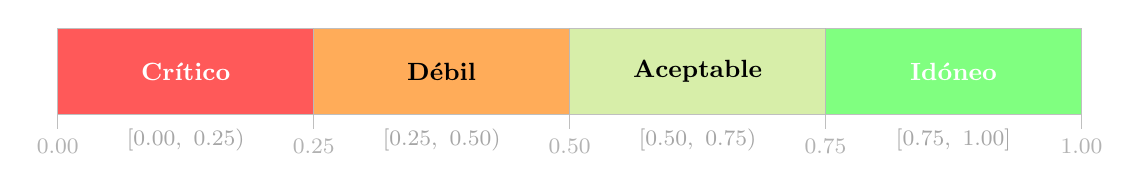
\begin{tikzpicture}

% ================================================================
%  Barra principal — ancho 13 cm, alto 1.1 cm
%  Bandas: 0–3.25 / 3.25–6.50 / 6.50–9.75 / 9.75–13.00
% ================================================================
\fill[red!65]             (0.00, 0) rectangle ( 3.25, 1.10);
\fill[orange!65]          (3.25, 0) rectangle ( 6.50, 1.10);
\fill[yellow!55!green!35] (6.50, 0) rectangle ( 9.75, 1.10);
\fill[green!50]           (9.75, 0) rectangle (13.00, 1.10);
\draw[gray!50, thin]      (0.00, 0) rectangle (13.00, 1.10);
\draw[gray!55, thin] (3.25, 0) -- (3.25, 1.10);
\draw[gray!55, thin] (6.50, 0) -- (6.50, 1.10);
\draw[gray!55, thin] (9.75, 0) -- (9.75, 1.10);

% Etiquetas de banda (centradas en cada zona)
\node[font=\small\bfseries, white]           at (1.625, 0.55) {Crítico};
\node[font=\small\bfseries]                  at (4.875, 0.55) {Débil};
\node[font=\small\bfseries]                  at (8.125, 0.55) {Aceptable};
\node[font=\small\bfseries, white]           at (11.375, 0.55) {Idóneo};

% Rangos numéricos debajo de cada banda
\node[font=\footnotesize, color=gray!70, anchor=north] at (1.625, -0.05)
    {$[0.00,\ 0.25)$};
\node[font=\footnotesize, color=gray!70, anchor=north] at (4.875, -0.05)
    {$[0.25,\ 0.50)$};
\node[font=\footnotesize, color=gray!70, anchor=north] at (8.125, -0.05)
    {$[0.50,\ 0.75)$};
\node[font=\footnotesize, color=gray!70, anchor=north] at (11.375, -0.05)
    {$[0.75,\ 1.00]$};

% Ticks en los puntos de corte
\foreach \xval in {0.00, 3.25, 6.50, 9.75, 13.00}{
    \draw[gray!50] (\xval, 0) -- (\xval, -0.18);
}
\node[font=\footnotesize, color=gray!60, anchor=north] at (0.00,  -0.18) {$0.00$};
\node[font=\footnotesize, color=gray!60, anchor=north] at (3.25,  -0.18) {$0.25$};
\node[font=\footnotesize, color=gray!60, anchor=north] at (6.50,  -0.18) {$0.50$};
\node[font=\footnotesize, color=gray!60, anchor=north] at (9.75,  -0.18) {$0.75$};
\node[font=\footnotesize, color=gray!60, anchor=north] at (13.00, -0.18) {$1.00$};

\end{tikzpicture}

\caption[Escala Garibelt: espectro de cuatro bandas de diagnóstico]{%
    Escala Garibelt: distribución del intervalo $[0,1]$ en cuatro bandas
    de diagnóstico territorial. Cada dimensión del Espectro MJG recibe
    una banda según su valor normalizado.}
\label{fig:escala-garibelt-barra}
\fuentefigura{Elaboración propia.}
\end{figure}

% =====================================================================
\subsubsection{Qué pregunta responde cada dimensión}
\label{subsubsec:garibelt-preguntas}
% =====================================================================

Para leer el Espectro MJG sin necesidad de conocer los detalles
computacionales, conviene tener presente qué pregunta urbana responde
cada dimensión:
\begin{itemize}
    \item Cobertura~$C$: ¿cuánto del área metropolitana queda dentro del
          radio de caminata de la red?
    \item Fuerza capilar~$C_i$: ¿qué tan variadas son las opciones de
          conexión disponibles en cada nodo?
    \item Índice de ruta directa~$DI$: ¿obliga la red a recorrer
          trayectos muy alejados de la distancia mínima?
    \item Tiempo promedio~$T$: ¿cuánto dura un viaje típico de extremo
          a extremo de la red?
    \item Intermediación~$B(v)$: ¿depende el flujo de la red de unos
          pocos nodos críticos o está distribuido entre muchos?
\end{itemize}
Cada banda del Espectro se lee como la respuesta a esa pregunta: Crítico
significa que la respuesta es desfavorable en grado severo; Idóneo,
que la red cumple con solidez estructural en esa dimensión.

% =====================================================================
\subsubsection{El procedimiento de normalización}
\label{subsubsec:garibelt-procedimiento}
% =====================================================================

Llevar un valor bruto a la escala $[0, 1]$ de la Clasificación Garibelt
requiere un rango de referencia. Para~$T$, ese rango lo entrega la
\textsc{enoe}: los tiempos de traslado en la \cdmx{} oscilan en la
práctica entre 85 y 180 minutos, de modo que 85 min normaliza a $1.0$
(Idóneo) y 180 min a $0.0$ (Crítico). Para~$DI$, la teoría de grafos
fija el piso en $1.0$ ---ruta directa perfecta--- y la práctica urbana
establece el techo en $2.5$ ---desviación que ya resulta inaceptable
para el usuario. Para~$C$, el estándar peatonal urbano de 80\,\% es la
referencia. Para~$C_i$, el rango es el del propio dataset: los
percentiles Q1 y Q3 de la distribución de grado nodal. Para~$B(v)$,
se calcula el índice de Gini de la distribución completa de
intermediación y se invierte: Gini~$= 0$ (distribución perfecta) da
$1.0$; Gini cercano a $1$ (monopolio) da $0.0$. La
la Tabla~\ref{tab:clasificacion-garibelt-dims} consolida estos rangos.

% =====================================================================
\subsubsection{Un tablero, no un marcador}
\label{subsubsec:garibelt-tablero}
% =====================================================================

Una ciudad puede cubrir la cuota legal de suministro de agua y tener,
al mismo tiempo, colonias con presión insuficiente, cortes en horas punta
y parámetros de saneamiento fuera de norma. Un clasificador escalar único
---«porcentaje de cobertura hídrica»--- tendería a ocultar esos puntos de
falla detrás de un valor promedio que parece satisfactorio. El transporte
metropolitano enfrenta el mismo problema de escala: la red puede mostrar
tiempos de viaje razonables y, en paralelo, tener toda su carga
concentrada en dos o tres nodos que la vuelven estructuralmente frágil.
La Clasificación Garibelt mantiene las cinco dimensiones separadas
precisamente para no perder esa información. \citet{deng2023} articulan
el principio como \termino{Safe-to-Fail}: evaluar una red es localizar
sus vulnerabilidades, no suavizarlas en un promedio. La subsección
siguiente presenta el procedimiento con un ejemplo hipotético.

% !TeX root = ../../../tesis.tex

% =====================================================================
\subsubsection{Ejemplo ilustrativo: Red Hipotética~\texorpdfstring{$\alpha$}{α}}
\label{subsubsec:garibelt-ejemplo}
% =====================================================================

La Figura~\ref{fig:garibelt-perfil-hipotetico} recorre el procedimiento
completo con la Red Hipotética~$\alpha$, cuyos valores son ilustrativos.
El perfil muestra lo que el instrumento está diseñado para detectar:
cobertura sólida en el territorio, pero eficiencia de ruta, fluidez y
distribución de carga en la banda Débil. Si esta fuera la red real de
una ciudad, el diagnóstico señalaría que el problema no es de alcance
---la red llega--- sino de calidad del servicio una vez dentro de la red.

\begin{figure}[htbp]
\centering
% Diagrama: Perfil ilustrativo — Red Hipotética α (Espectro MJG)
% Usado en: 3-Conceptos-Indicadores/3-3-Indicadores/3-3-9-Clasificacion-Garibelt/3-3-9-3-Ejemplo.tex
% fig:garibelt-perfil-hipotetico
%
% Cinco filas horizontales (una por dimensión). Fondo de bandas en tono claro,
% círculo marcador al valor normalizado, etiquetas izquierda y derecha.
% Valores de Red α: C=0.85, C_i=0.60, DI=0.40, T=0.42, B(v)=0.30
% Barra: x in [0,6]; 4 bandas en x=1.5/3.0/4.5; dy=1.0; bh=0.60

\tikzsetnextfilename{garibelt-perfil-hipotetico}
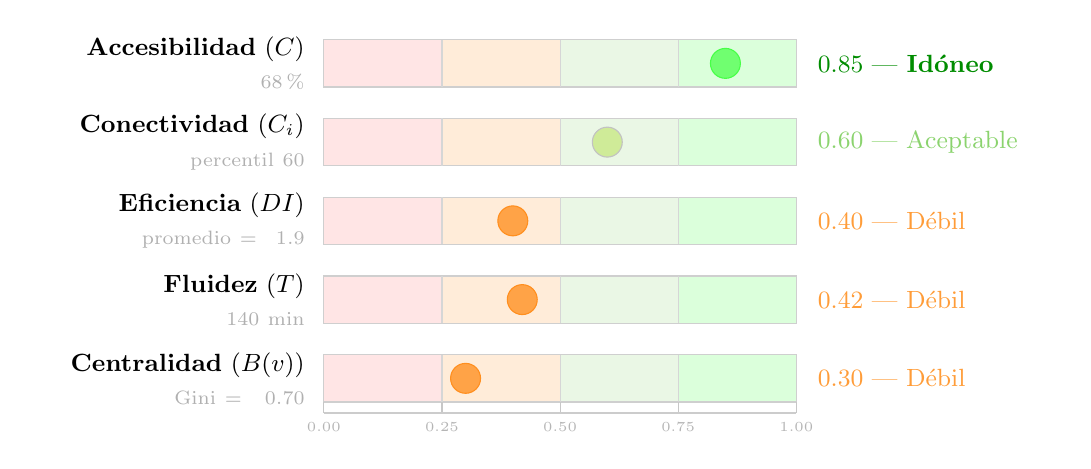
\begin{tikzpicture}[
    etiq/.style = {
        font       = \small,
        align      = right,
        text width = 3.4cm
    },
    vallab/.style = {
        font       = \small,
        align      = left,
        text width = 3.0cm,
        anchor     = west
    }
]

% ================================================================
%  FONDOS DE BANDA + BORDES (5 filas)
%  Fila n: y_base = n*1.0;  y_top = y_base + 0.60
%  Divisores de banda en x = 1.5 / 3.0 / 4.5
% ================================================================

\foreach \yb in {0, 1, 2, 3, 4}{
    \fill[red!10]              (0.0, \yb)   rectangle (1.5, \yb+0.60);
    \fill[orange!15]           (1.5, \yb)   rectangle (3.0, \yb+0.60);
    \fill[yellow!18!green!10]  (3.0, \yb)   rectangle (4.5, \yb+0.60);
    \fill[green!14]            (4.5, \yb)   rectangle (6.0, \yb+0.60);
    \draw[gray!38, thin]       (0.0, \yb)   rectangle (6.0, \yb+0.60);
    \draw[gray!32, thin]       (1.5, \yb)   -- (1.5,  \yb+0.60);
    \draw[gray!32, thin]       (3.0, \yb)   -- (3.0,  \yb+0.60);
    \draw[gray!32, thin]       (4.5, \yb)   -- (4.5,  \yb+0.60);
}

% ================================================================
%  MARCADORES (círculos rellenos con color de su banda)
%  x = valor_norm × 6 ;  y = y_base + 0.30 (centro de fila)
% ================================================================

% Fila 0 — Centralidad B(v): norm=0.30 → x=1.80 — Débil
\fill[orange!72] (1.80, 0.30) circle (0.19);
\draw[orange!88, thin] (1.80, 0.30) circle (0.19);

% Fila 1 — Fluidez T: norm=0.42 → x=2.52 — Débil
\fill[orange!72] (2.52, 1.30) circle (0.19);
\draw[orange!88, thin] (2.52, 1.30) circle (0.19);

% Fila 2 — Eficiencia DI: norm=0.40 → x=2.40 — Débil
\fill[orange!72] (2.40, 2.30) circle (0.19);
\draw[orange!88, thin] (2.40, 2.30) circle (0.19);

% Fila 3 — Conectividad C_i: norm=0.60 → x=3.60 — Aceptable
\fill[yellow!55!green!42] (3.60, 3.30) circle (0.19);
\draw[gray!48, thin] (3.60, 3.30) circle (0.19);

% Fila 4 — Accesibilidad C: norm=0.85 → x=5.10 — Idóneo
\fill[green!56] (5.10, 4.30) circle (0.19);
\draw[green!72, thin] (5.10, 4.30) circle (0.19);

% ================================================================
%  ETIQUETAS IZQUIERDA
%  dimensión (negrita) en línea 1, valor bruto en línea 2
% ================================================================

\node[etiq, anchor=east] at (-0.12, 0.30)
    {\textbf{Centralidad} ($B(v)$)\\[1pt]
     \textcolor{gray!62}{\scriptsize Gini~$= 0.70$}};

\node[etiq, anchor=east] at (-0.12, 1.30)
    {\textbf{Fluidez} ($T$)\\[1pt]
     \textcolor{gray!62}{\scriptsize 140 min}};

\node[etiq, anchor=east] at (-0.12, 2.30)
    {\textbf{Eficiencia} ($DI$)\\[1pt]
     \textcolor{gray!62}{\scriptsize promedio $= 1.9$}};

\node[etiq, anchor=east] at (-0.12, 3.30)
    {\textbf{Conectividad} ($C_i$)\\[1pt]
     \textcolor{gray!62}{\scriptsize percentil 60}};

\node[etiq, anchor=east] at (-0.12, 4.30)
    {\textbf{Accesibilidad} ($C$)\\[1pt]
     \textcolor{gray!62}{\scriptsize 68\,\%}};

% ================================================================
%  ETIQUETAS DERECHA (valor normalizado — banda)
% ================================================================

\node[vallab, color=orange!78] at (6.15, 0.30) {$0.30$ — Débil};
\node[vallab, color=orange!78] at (6.15, 1.30) {$0.42$ — Débil};
\node[vallab, color=orange!78] at (6.15, 2.30) {$0.40$ — Débil};
\node[vallab, color=yellow!30!green!65] at (6.15, 3.30) {$0.60$ — Aceptable};
\node[vallab, color=green!55!black]     at (6.15, 4.30) {$0.85$ — \textbf{Idóneo}};

% ================================================================
%  EJE DE ESCALA INFERIOR
% ================================================================

\foreach \xval/\lab in {0.0/0.00, 1.5/0.25, 3.0/0.50, 4.5/0.75, 6.0/1.00}{
    \draw[gray!44] (\xval, 0.0) -- (\xval, -0.14);
    \node[font=\tiny, color=gray!58, anchor=north] at (\xval, -0.14) {\lab};
}

% Línea de eje
\draw[gray!40] (0.0, -0.14) -- (6.0, -0.14);

\end{tikzpicture}

\caption[Perfil ilustrativo de la Clasificación Garibelt: Red Hipotética~$\alpha$]{%
    Perfil Garibelt de la Red Hipotética~$\alpha$. Cada fila corresponde a
    una dimensión del Espectro MJG; el círculo indica el valor normalizado
    y su posición en la Escala Garibelt. Los valores son ilustrativos.}
\label{fig:garibelt-perfil-hipotetico}
\fuentefigura{Elaboración propia.}
\end{figure}

De los ocho indicadores del capítulo, dos quedan fuera de la versión~1
del instrumento. $W_{s,h}$ (Penalización por Transferencia) tiene
implementación parcial en el motor \termino{VFTModel}; su incorporación
queda diferida a la versión~2. $\Delta E$ (Robustez Geométrica) requiere
múltiples corridas del grafo con nodos removidos, operación que
corresponde a la Fase~4 y está fuera del alcance del presente análisis.
La aplicación del instrumento a la red de la \zmvm{} ---incluyendo los
valores normalizados y la lectura por dimensión--- se presenta en la
\autoref{sec:diagnostico-garibelt} del \autoref{ch:analisis-red-actual}.

